\section{三角形网格}\label{sec:三角形网格}
\keyindex{三角形}{triangle}{}是计算机图形学最常用的形状;
复杂场景会用上百万三角形建模以实现出色细节
(\reffig{3.11}展示了四百多万三角形的复杂三角网格图像)。
\begin{figure}[htbp]
    \centering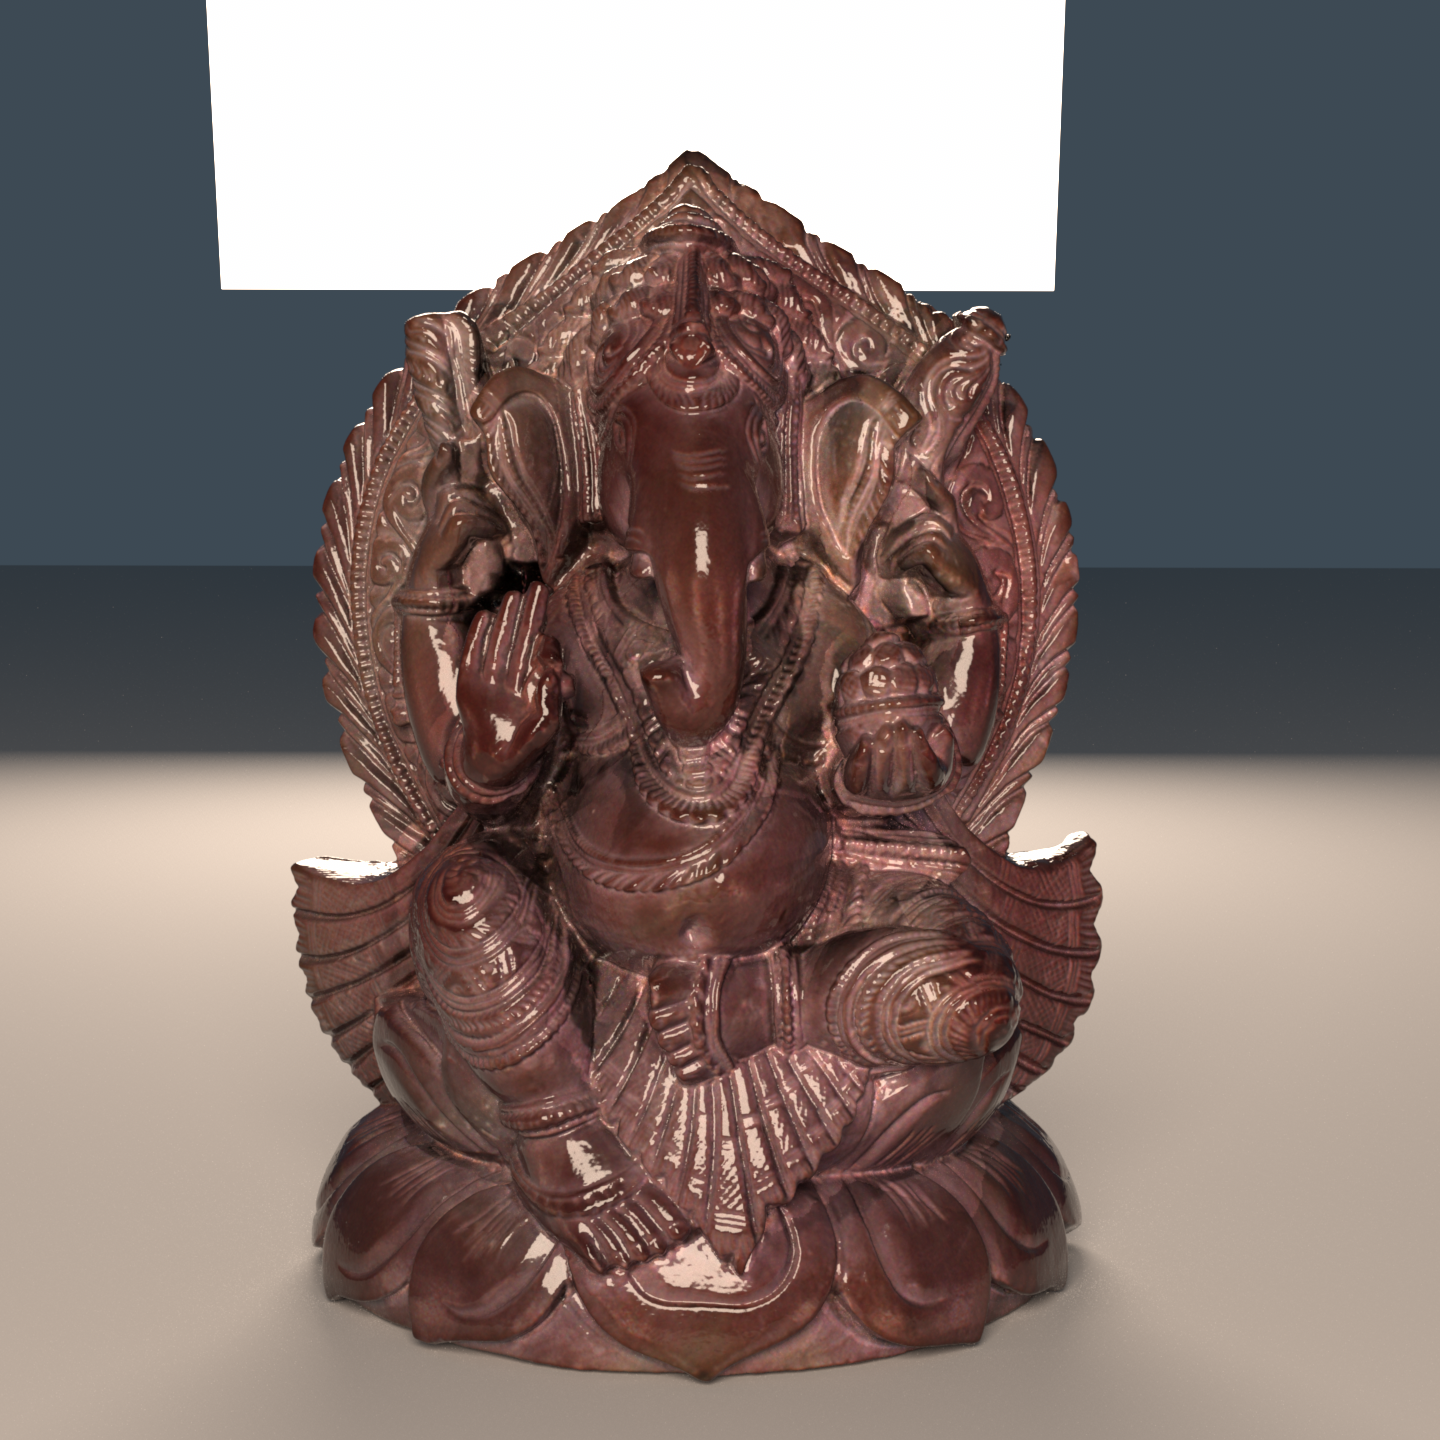
\includegraphics[width=\linewidth]{chap03/ganesha.png}
    \caption{象头神模型。该三角网格含有四百多万个独立三角形。
        它是使用结构光确定物体形状的3D扫描器用真实雕塑创建的。}
    \label{fig:3.11}
\end{figure}

尽管自然的表示是用{\ttfamily Triangle}形状实现,
每个三角形都存储它三个顶点的位置,
但内存更高效的表示是用一个顶点位置数组分开存储整个\keyindex{三角网格}{triangle mesh}{},
每个独立三角形只存储它三个顶点对该数组的三个偏移量。

为了理解为什么是这样,考虑著名的\keyindex{欧拉-庞加莱公式}{Euler-Poincaré formula}{},
它将闭合离散网格的顶点数$V$、边数$E$和面数$F$联系起来:
\begin{align*}
    V-E+F=2(1-g)\, ,
\end{align*}
其中$g\in\mathbb{N}$是网格的\keyindex{亏格}{genus}{}。
亏格通常是很小的数且能解释为网格的“手柄”数量(类似于茶杯把手)。
在三角网格上,边数和面数\sidenote{译者注:原文错写为顶点数,已修改。}还由恒等式联系
\begin{align*}
    E=\frac{3}{2}F\, .
\end{align*}
这可以看作把每条边分成两部分与两个相邻三角形关联。
有$3F$条这样的半边,所有同位的边对构成$E$条网格边。
对于巨大的闭合三角网格,亏格的整体影响通常可以忽略,
我们可以结合之前两个方程(以及$g=0$)得到
\begin{align*}
    F\approx2V\, .
\end{align*}
换句话说,面数大约是顶点数的两倍。
既然每个面引用三个顶点,每个顶点(平均)总共被引用六次。
因此当共享顶点时,每个三角形所需的总分摊存储为
偏移量的12字节内存(三个4字节32位整数偏移量)加上一个顶点存储的一半——6字节,
这里假设每个顶点用三个4字节浮点存储——每个三角形一共18字节。
这比每个三角形直接用36字节存储三个位置好得多。
当网格中有每个顶点的曲面法线或纹理坐标时,相对的存储节约会更好。

pbrt使用结构体\refvar{TriangleMesh}{}保存关于三角网格的共享信息。
\begin{lstlisting}
`\initcode{Triangle Declarations}{=}\initnext{TriangleDeclarations}`
struct `\initvar{TriangleMesh}{}` {
    `\refcode{TriangleMesh Public Methods}{}`
    `\refcode{TriangleMesh Data}{}`
};
\end{lstlisting}
\begin{lstlisting}
`\initcode{TriangleMesh Public Methods}{=}`
`\refvar{TriangleMesh}{}`(const `\refvar{Transform}{}` &ObjectToWorld, int nTriangles, const int *vertexIndices,
    int nVertices, const `\refvar{Point3f}{}` *P, const `\refvar{Vector3f}{}` *S, const `\refvar{Normal3f}{}` *N,
    const `\refvar{Point2f}{}` *uv, const std::shared_ptr<`\refvar{Texture}{}`<`\refvar{Float}{}`>> &alphaMask);
\end{lstlisting}

\refvar{TriangleMesh}{}构造函数的参数如下:
\begin{itemize}
    \item {\ttfamily ObjectToWorld}:网格的物体到世界的变换。
    \item {\ttfamily nTriangles}:网格中三角形总数。
    \item {\ttfamily vertexIndices}:指向顶点索引数组的指针。对于第{\ttfamily i}个三角形,其三个顶点位置为
          {\ttfamily P[vertexIndices[3*i]]}、{\ttfamily P[vertexIndices[3*i+1]]}和{\ttfamily P[vertexIndices[3*i+2]]}。
    \item {\ttfamily nVertices}:网格中顶点总数。
    \item {\ttfamily P}:{\ttfamily nVertices}个顶点位置的数组。
    \item {\ttfamily S}:可选切向量数组,网格中每个顶点都有一个。它们用于计算着色切线。
    \item {\ttfamily N}:可选法向量数组,网格中每个顶点都有一个。如果有,则它们在三角形面之间插值以计算着色法线。
    \item {\ttfamily UV}:可选参数值$(u,v)$数组,每个顶点一个。
    \item {\ttfamily alphaMask}:可选的\keyindex{$\alpha$掩模}{alpha mask}{}纹理,可用于截去部分三角形面。
\end{itemize}

pbrt中三角形在形状里有双重角色:不仅场景描述文件经常直接指定它们,
其他形状也常把自己细分为三角网格。
例如,细分曲面最终创建一个三角网格来近似光滑有限曲面。
再对这些三角形执行光线相交,而不是直接对细分曲面这样做(\refsub{细分})。

由于这第二种角色,创建三角网格的代码能指定三角形的参数化很重要。
如果三角形是通过求取参数化曲面在三个特定坐标值$(u,v)$处的位置来创建的,
这些$(u,v)$值应该被插值以计算三角形内光线交点处的$(u,v)$值。
显式指定$(u,v)$值对纹理贴图也很有用,创建三角网格的外部程序
可能想给网格赋值$(u,v)$坐标,这样纹理贴图以期望的方式把颜色赋值给网格曲面。

\refvar{TriangleMesh}{}构造函数赋值相关信息并存于成员变量中。
特别地,它自己复制{\ttfamily vertexIndices、P、N、S}和{\ttfamily UV},
允许调用者保留对传入数据的所有权。
\begin{lstlisting}
`\initcode{Triangle Method Definitions}{=}\initnext{TriangleMethodDefinitions}`
`\refvar{TriangleMesh}{}`::`\refvar{TriangleMesh}{}`(const `\refvar{Transform}{}` &ObjectToWorld,
        int nTriangles, const int *vertexIndices, int nVertices,
        const `\refvar{Point3f}{}` *P, const `\refvar{Vector3f}{}` *S, const `\refvar{Normal3f}{}` *N,
        const `\refvar{Point3f}{}` *UV,
        const std::shared_ptr<`\refvar{Texture}{}`<`\refvar{Float}{}`>> &alphaMask)
    : `\refvar{nTriangles}{}`(nTriangles), `\refvar{nVertices}{}`(nVertices), 
      `\refvar{vertexIndices}{}`(vertexIndices, vertexIndices + 3 * nTriangles),
      `\refvar{alphaMask}{}`(alphaMask) {
    `\refcode{Transform mesh vertices to world space}{}`
    `\refcode{Copy UV, N, and S vertex data, if present}{}`
}
\end{lstlisting}
\begin{lstlisting}
    `\initcode{TriangleMesh Data}{=}`
    const int `\initvar{nTriangles}{}`, `\initvar{nVertices}{}`;
    std::vector<int> `\initvar{vertexIndices}{}`;
    std::unique_ptr<`\refvar{Point3f}{}`[]> `\initvar[TriangleMesh::p]{p}{}`;
    std::unique_ptr<`\refvar{Normal3f}{}`[]> `\initvar[TriangleMesh::n]{n}{}`;
    std::unique_ptr<`\refvar{Vector3f}{}`[]> `\initvar[TriangleMesh::s]{s}{}`;
    std::unique_ptr<`\refvar{Point2f}{}`[]> `\initvar[TriangleMesh::uv]{uv}{}`;
    std::shared_ptr<`\refvar{Texture}{}`<`\refvar{Float}{}`>> `\initvar{alphaMask}{}`;
\end{lstlisting}

不像其他形状那样把形状描述留在物体空间内然后
将入射光线从世界空间变换到物体空间,
三角网格将形状变换到世界空间,
因此节约了把入射光线变换到物体空间的工作和
把相交处的几何表示变换出世界空间的工作。
这是个好主意,因为该操作可在启动后执行,
避免渲染中多次变换光线。
尽管也能对二次曲面使用该方法,但会更复杂(见本章末习题7了解更多信息)。
\begin{lstlisting}
    `\initcode{Transform mesh vertices to world space}{=}`
    `\refvar[TriangleMesh::p]{p}{}`.reset(new `\refvar{Point3f}{}`[`\refvar{nVertices}{}`]);
    for (int i = 0; i < `\refvar{nVertices}{}`; ++i)
    `\refvar[TriangleMesh::p]{p}{}`[i] = ObjectToWorld(P[i]);
\end{lstlisting}

代码片\refcode{Copy UV, N, and S vertex data, if present}{}只是
分配合适数量的空间并复制合适的值。
如果有法线和切向量,则也变换到世界空间。
\begin{lstlisting}
`\initcode{Copy UV, N, and S vertex data, if present}{=}`
if (UV) {
    `\refvar[TriangleMesh::uv]{uv}{}`.reset(new `\refvar{Point2f}{}`[`\refvar{nVertices}{}`]);
    memcpy(`\refvar[TriangleMesh::uv]{uv}{}`.get(), UV, `\refvar{nVertices}{}` * sizeof(`\refvar{Point2f}{}`));
}
if (N) {
    `\refvar[TriangleMesh::n]{n}{}`.reset(new `\refvar{Normal3f}{}`[`\refvar{nVertices}{}`]);
    for (int i = 0; i < `\refvar{nVertices}{}`; ++i)
        `\refvar[TriangleMesh::n]{n}{}`[i] = ObjectToWorld(N[i]);
}
if (S) {
    `\refvar[TriangleMesh::s]{s}{}`.reset(new `\refvar{Vector3f}{}`[`\refvar{nVertices}{}`]);
    for (int i = 0; i < `\refvar{nVertices}{}`; ++i)
        `\refvar[TriangleMesh::s]{s}{}`[i] = ObjectToWorld(S[i]);
}
\end{lstlisting}

\subsection{三角形}\label{sub:三角形}
类\refvar{Triangle}{}实际上实现了\refvar{Shape}{}接口。它表示单个三角形。
\begin{lstlisting}
`\refcode{Triangle Declarations}{+=}\lastcode{TriangleDeclarations}`
class `\initvar{Triangle}{}` : public `\refvar{Shape}{}` {
public:
    `\refcode{Triangle Public Methods}{}`
private:
    `\refcode{Triangle Private Methods}{}`
    `\refcode{Triangle Private Data}{}`
};
\end{lstlisting}

\refvar{Triangle}{}不存储太多数据——只有一个指向其来处的父\refvar{TriangleMesh}{}指针
和一个指向网格中其三个顶点索引的指针。
\begin{lstlisting}
`\initcode{Triangle Public Methods}{=}`
`\refvar{Triangle}{}`(const `\refvar{Transform}{}` *ObjectToWorld, const `\refvar{Transform}{}` *WorldToObject,
         bool reverseOrientation,
         const std::shared_ptr<`\refvar{TriangleMesh}{}`> &mesh, int triNumber)
    : `\refvar{Shape}{}`(ObjectToWorld, WorldToObject, reverseOrientation),
      `\refvar{mesh}{}`(mesh) {
    `\refvar[Triangle::v]{v}{}` = &mesh->`\refvar{vertexIndices}{}`[3 * triNumber];
}
\end{lstlisting}

注意该实现存储了指向第一个顶点\emph{索引}的指针,
而非存储三个指向顶点自己的指针。
这以另一级别的间接性为代价减少了每个\refvar{Triangle}{}所需的存储量。
\begin{lstlisting}
`\initcode{Triangle Private Data}{=}`
std::shared_ptr<`\refvar{TriangleMesh}{}`> `\initvar{mesh}{}`;
const int *`\initvar[Triangle::v]{v}{}`;
\end{lstlisting}

因为pbrt中大量的其他形状表示会把自己转化为三角网格,
实用函数
\refvar{CreateTriangleMesh}{()}仔细创建
底层\refvar{TriangleMesh}{}以及网格中每个三角形的\refvar{Triangle}{}。
它返回三角形状的向量。
\begin{lstlisting}
`\refcode{Triangle Method Definitions}{+=}\lastnext{TriangleMethodDefinitions}`
std::vector<std::shared_ptr<`\refvar{Shape}{}`>> `\initvar{CreateTriangleMesh}{}`(
        const `\refvar{Transform}{}` *ObjectToWorld, const `\refvar{Transform}{}` *WorldToObject,
        bool reverseOrientation, int nTriangles,
        const int *vertexIndices, int nVertices, const `\refvar{Point3f}{}` *p,
        const `\refvar{Vector3f}{}` *s, const `\refvar{Normal3f}{}` *n, const `\refvar{Point2f}{}` *uv,
        const std::shared_ptr<`\refvar{Texture}{}`<`\refvar{Float}{}`>> &alphaMask) {
    std::shared_ptr<`\refvar{TriangleMesh}{}`> mesh = std::make_shared<`\refvar{TriangleMesh}{}`>(
        *ObjectToWorld, nTriangles, vertexIndices, nVertices, p, s, n, uv,
        alphaMask);
    std::vector<std::shared_ptr<`\refvar{Shape}{}`>> tris;
    for (int i = 0; i < nTriangles; ++i)
        tris.push_back(std::make_shared<`\refvar{Triangle}{}`>(ObjectToWorld,
            WorldToObject, reverseOrientation, mesh, i));
    return tris;
}
\end{lstlisting}

三角形的物体空间边界很容易通过计算包围其三个顶点的边界框求得。
因为顶点位置\refvar[TriangleMesh::p]{p}{}在构造函数中被变换到世界空间,
这里的实现要在计算其边界前把它们变换回物体空间。
\begin{lstlisting}
`\refcode{Triangle Method Definitions}{+=}\lastnext{TriangleMethodDefinitions}`
`\refvar{Bounds3f}{}` `\refvar{Triangle}{}`::`\initvar[Triangle::ObjectBound]{\refvar{ObjectBound}{}}{}`() const {
    `\refcode{Get triangle vertices in p0, p1, and p2}{}`
    return `\refvar[Union1]{Union}{}`(`\refvar{Bounds3f}{}`((*`\refvar{WorldToObject}{}`)(p0), (*`\refvar{WorldToObject}{}`)(p1)),
                 (*`\refvar{WorldToObject}{}`)(p2));
}
\end{lstlisting}
\begin{lstlisting}
`\initcode{Get triangle vertices in p0, p1, and p2}{=}`
const `\refvar{Point3f}{}` &p0 = `\refvar{mesh}{}`->`\refvar[TriangleMesh::p]{p}{}`[`\refvar[Triangle::v]{v}{}`[0]];
const `\refvar{Point3f}{}` &p1 = `\refvar{mesh}{}`->`\refvar[TriangleMesh::p]{p}{}`[`\refvar[Triangle::v]{v}{}`[1]];
const `\refvar{Point3f}{}` &p2 = `\refvar{mesh}{}`->`\refvar[TriangleMesh::p]{p}{}`[`\refvar[Triangle::v]{v}{}`[2]];
\end{lstlisting}

比起变换其物体空间边界框到世界空间,
\refvar{Triangle}{}形状是能计算更好的世界空间边界的形状之一。
其世界空间边界可以直接从世界空间顶点算得。
\begin{lstlisting}
`\refcode{Triangle Method Definitions}{+=}\lastnext{TriangleMethodDefinitions}`
`\refvar{Bounds3f}{}` `\refvar{Triangle}{}`::`\initvar[Triangle::WorldBound]{\refvar[Shape::WorldBound]{WorldBound}{}}{}`() const {
    `\refcode{Get triangle vertices in p0, p1, and p2}{}`
    return `\refvar[Union1]{Union}{}`(`\refvar{Bounds3f}{}`(p0, p1), p2); 
}
\end{lstlisting}

\subsection{三角形相交}\label{sub:三角形相交}
三角形状方法的\refvar[Triangle::Intersect]{Intersect}{()}结构
